\documentclass{article}
\usepackage[linktocpage=true]{hyperref}
\usepackage{graphicx}
\usepackage[T1]{fontenc} 
\usepackage[utf8]{inputenc}
\usepackage{subfigure}
\usepackage{color}
\def\todo#1{}%{{\color{red} #1}}
\def\fixme#1{}%{{\color{green} #1}}

\author{Loïc Simon}
\title{BSI TP3: Modèles d'illumination locale}
\date{\today}

\begin{document}
\maketitle

% Objectif<<<
L'objectif de ce TP est de mettre en place les modèles d'illumination simples,
\begin{itemize}
  \item modèle lambertien,
  \item modèle de Phong,
  \item modèle de Blinn-Phong,
\end{itemize}

ainsi que différentes implémentations,
\begin{itemize}
\item Gouraud,
\item Phong,
\item Bump mapping.
\end{itemize}

{\bf NB1:} Pour répondre aux exercices suivant vous travaillerez essentiellement dans les
fichiers de shaders \verb|illumination.v.glsl| et \verb|illumination.f.glsl|.
Toutefois, vous devrez au préalable copier le code de la fonction
\verb|loadTextureTGA_glfw| du TP précédent dans la fonction
\verb|loadTGATexture| du fichier \verb|utils/textures.cpp|.

{\bf NB2:} Par ailleurs, le TP étant assez long, vous êtes conviés a travailler
en parallèle au sein de votre binôme pour coder chacun une partie des modèles
d'illumination et des implémentations proposés. Vous rassemblerez votre code par la
suite (de préférence en utilisant git).
%>>>

\section{Exercices}

\subsection{Exercice 1: Modèle diffus Lambertien}%<<<

Dans les 2 fichiers GLSL, implémentez le modèle diffus lambertien dans la
fonction \verb|ComputeLightLambert|. Vous porterez une attention particulière au
repère choisi pour définir les diverses directions impliquées (normale,
lumière). Elles doivent évidemment être définies dans un repère commun.
\begin{itemize}
  \item[{\bf Q1.}] Commentez sur l'intérêt de ce type de rendu par rapport au modèle ambiant.
\end{itemize}
%>>>

\subsection{Exercice 2: Modèle spéculaire de Phong}%<<<

Dans le fichier \verb|illumination.v.glsl| (c-à-d le vertex shader) implémentez le modèle de Phong via la
fonction \verb|ComputeLightSpecular|.

\begin{itemize}
  \item[{\bf Q2.}] S'agit-il d'une implémentation de type Gouraud ou Phong? 
  \item[{\bf Q3.}] Critiquez les limitations de cette approche. Illustrez par des screenshots annotés.
\end{itemize}
%>>>

\subsection{Exercice 3: Modèle de Blinn-Phong}%<<<

Dans le fichier \verb|illumination.f.glsl| (c-à-d le fragment shader) implémentez le modèle de Blinn-Phong
via la fonction \verb|ComputeLightSpecular|. Attention le modèle de Blinn-Phong
n'a pas été traité en cours. Vous pourrez trouver les détails le concernant sur
Wikipedia:
\url{http://en.wikipedia.org/wiki/Blinn-Phong_shading_model}

\begin{itemize}
  \item[{\bf Q4.}] Vous devriez noter une nette amélioration des reflets spéculaires par
    rapport à l'exercice 2. A quoi est elle due, selon vous? Vous prendrez soin de différentier le cas du plan horizontal et de la tête de singe.
  \item[{\bf Q5.}] Tous les objets de la scène sont ils frappés par ce changement de manière égale? Si non, lesquels ne sont pas impactés et pourquoi?
\end{itemize}                         
%>>>

\subsection{Exercice 4 et 5: Bump Mapping}%<<<

\subsubsection{Théorie}

L'objectif du bump mapping est de représenter de façon simple mais réaliste le grain macroscopique d'un objet. Par exemple, pour un objet texturé, l'aspect d'un reflet obtenu par un shading de type Phong paraît peu réaliste car la courbure de la surface suggérée par les reflets est en désaccord avec celle induite par les variations de la texture (cf figure \ref{fig:bm} \subref{subfig:textured}).

Pour pallier à ce défaut, le bump mapping consiste à définir la normale en chaque fragment par le biais d'une texture, ce qui permet d'accorder les variations de la normale avec celle de la couleur (cf figure \ref{fig:bm} \subref{subfig:bumpMapped}). Ce type de texture constitue une carte de normales (ou \emph{normal map} en anglais).

\begin{figure}
  \subfigure[]{\label{subfig:textured}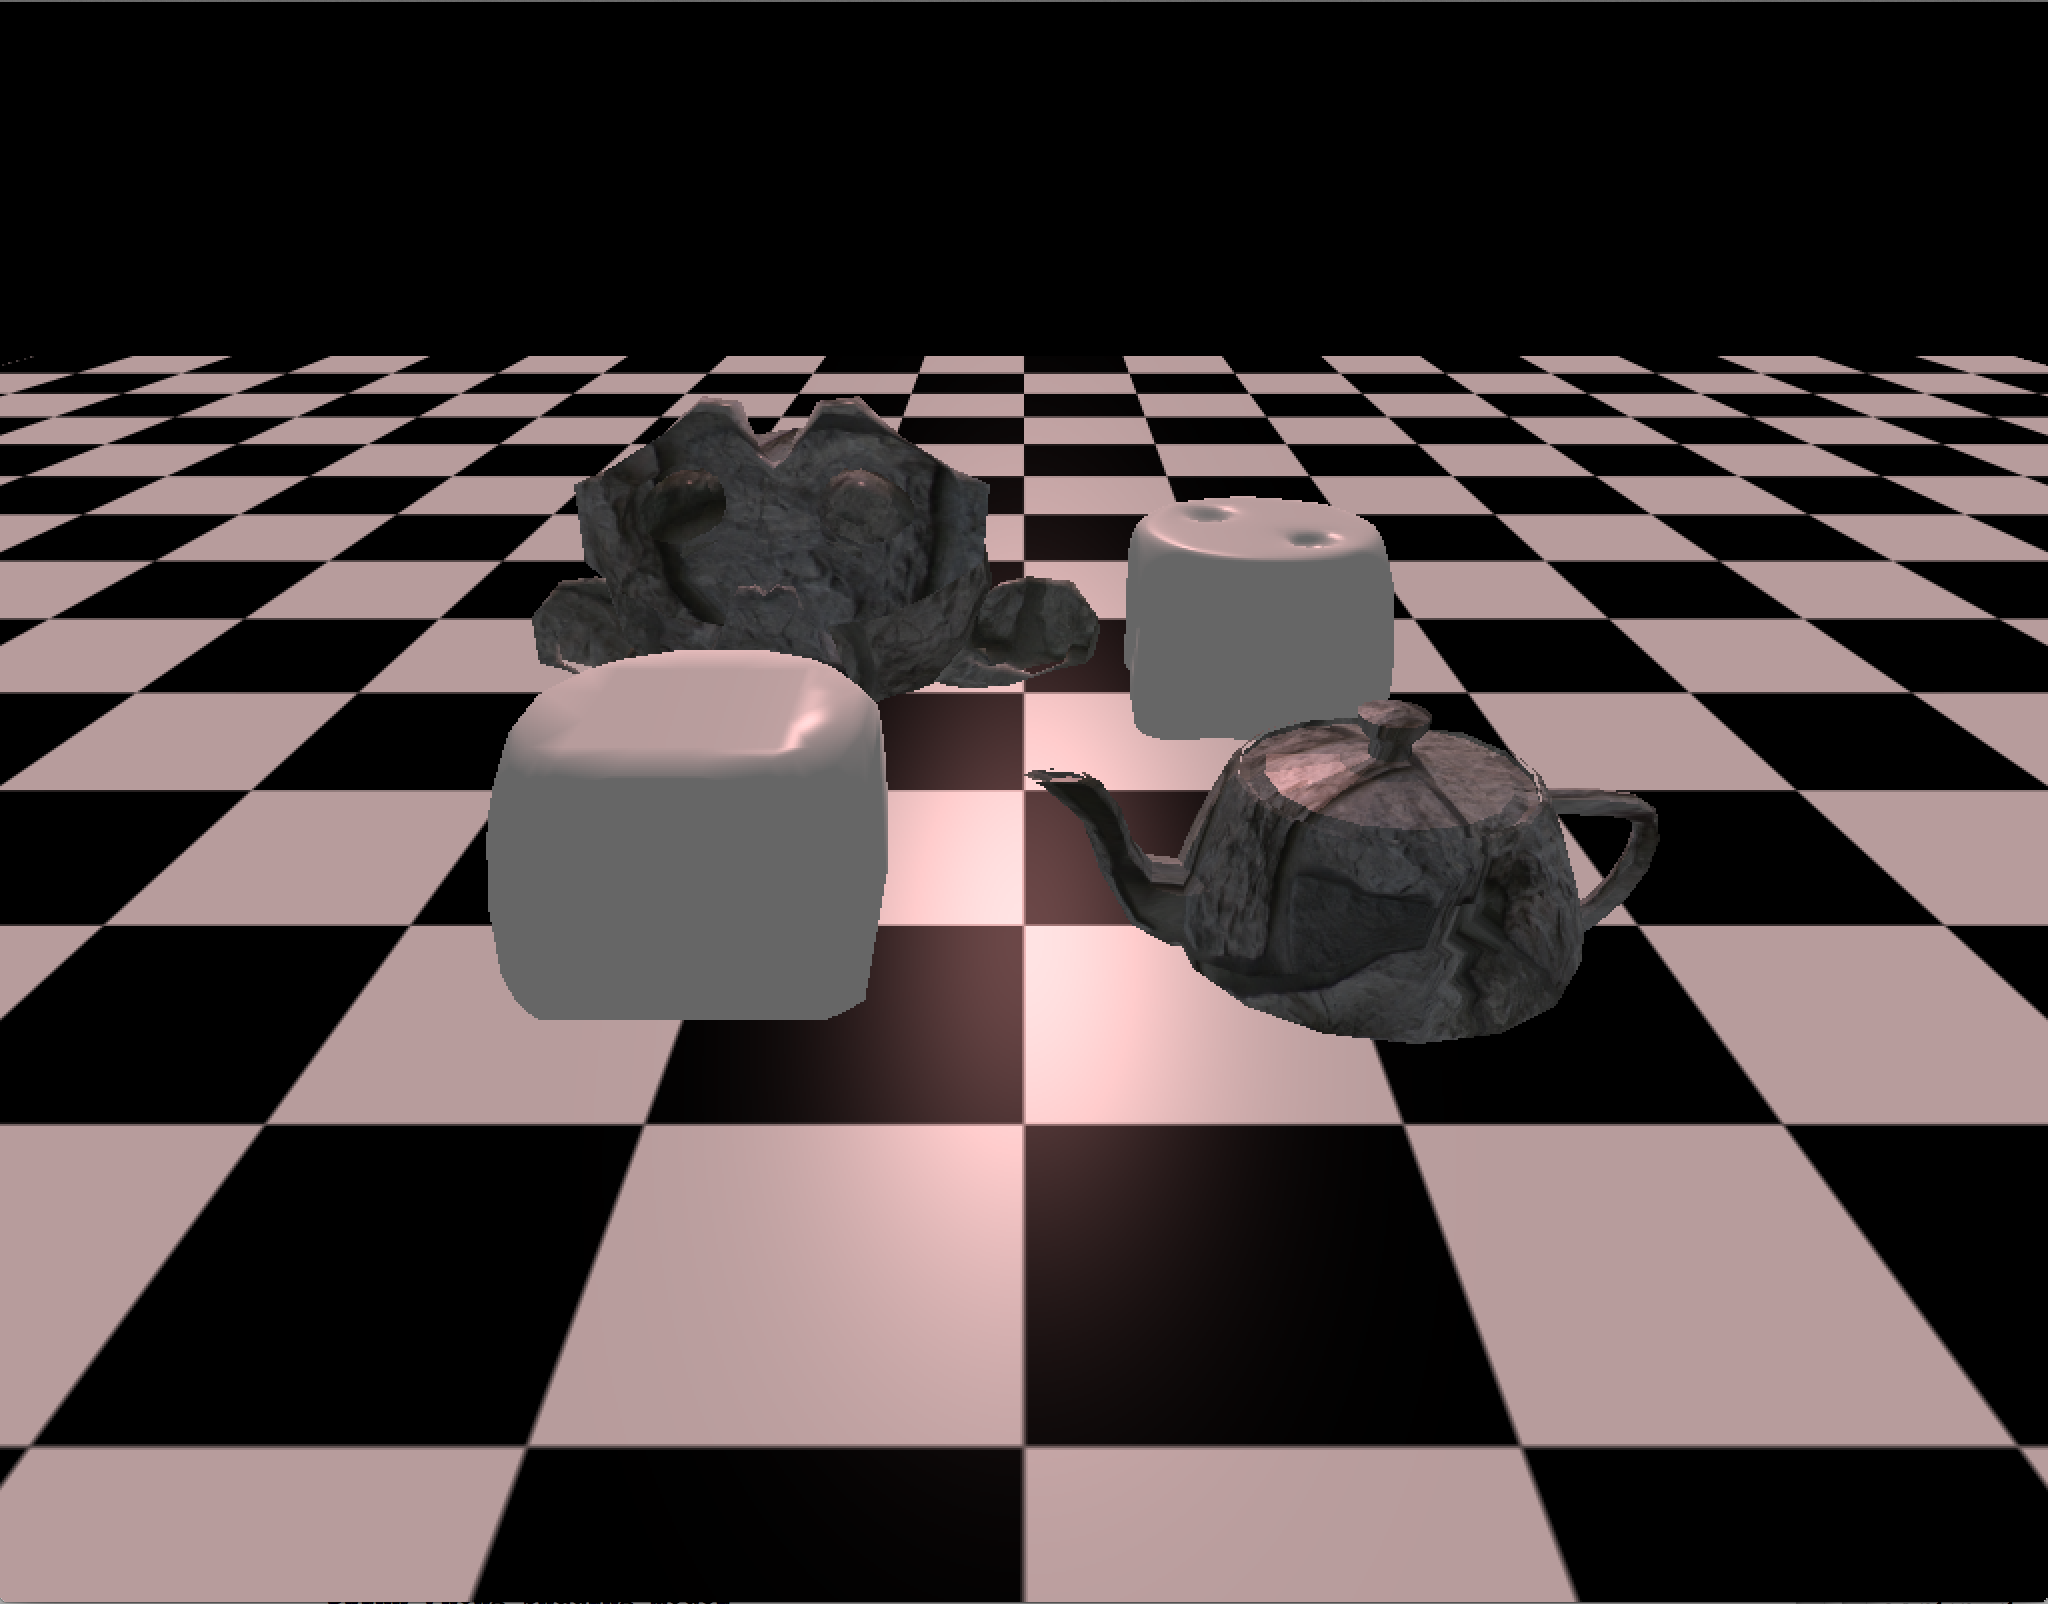
\includegraphics[width=0.5\textwidth]{images/textured}}
  \subfigure[]{\label{subfig:bumpMapped}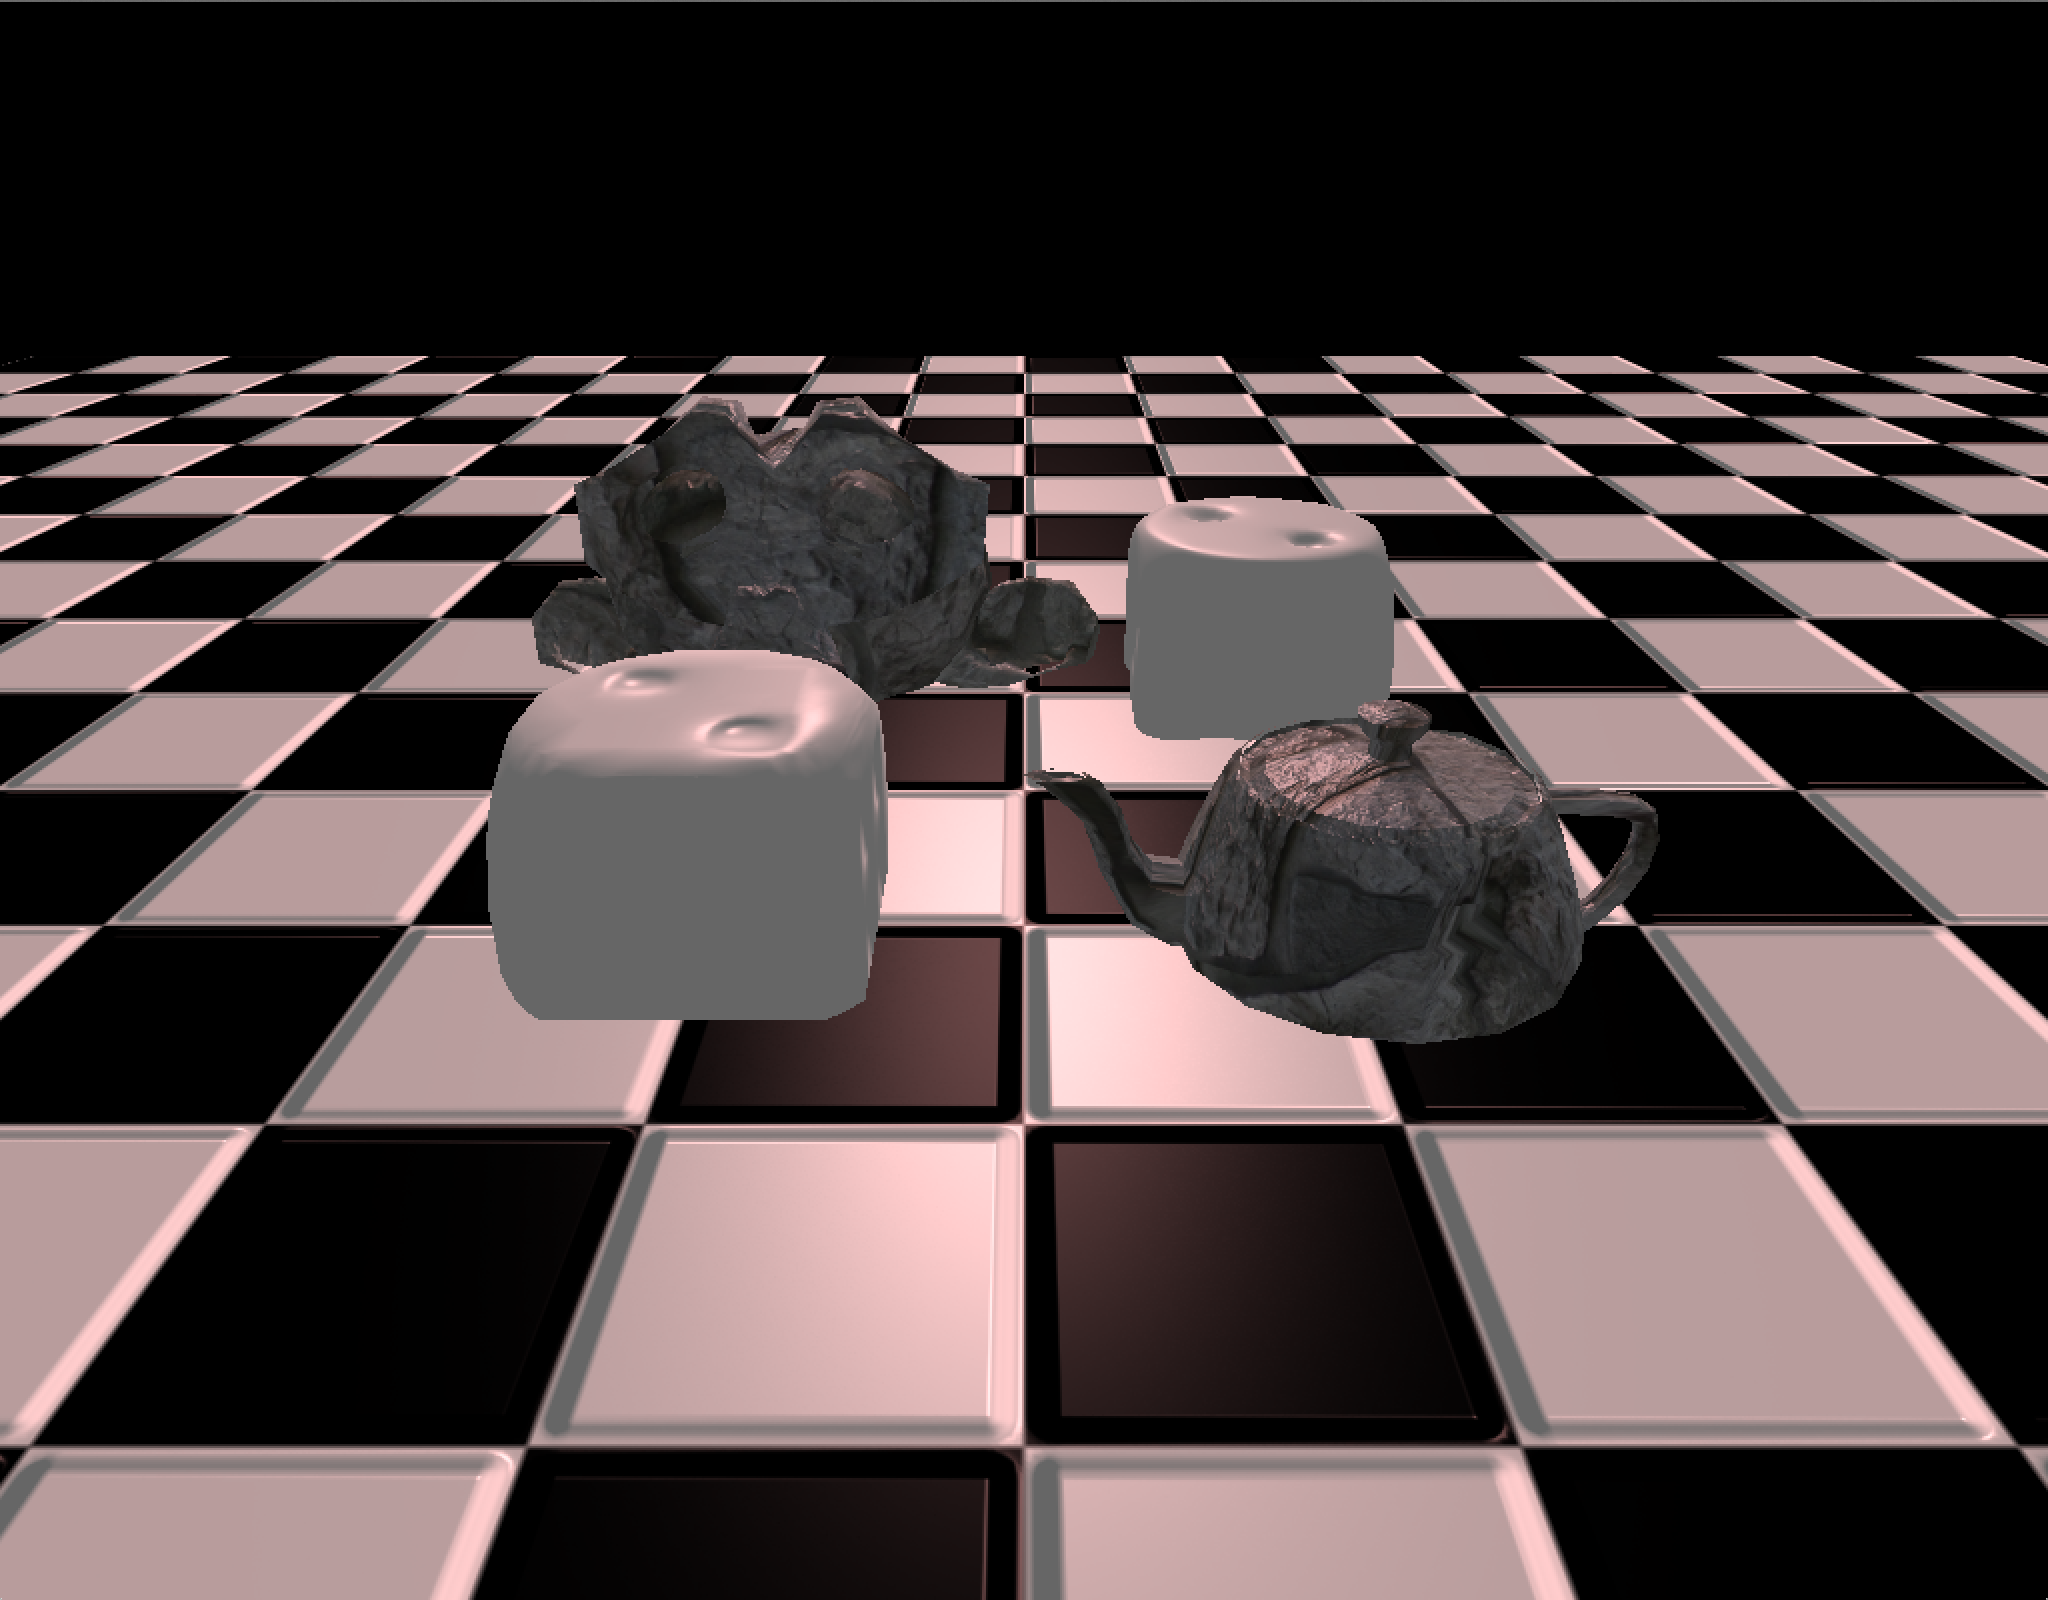
\includegraphics[width=0.5\textwidth]{images/bumpMapped}}
\caption{Scène texturée avec un reflet de type Blinn-Phong. Dans le deuxième cas, une technique de bump mapping a été utilisée.}
\label{fig:bm}
\end{figure}

\paragraph{Espace tangent}
Contrairement au cas des textures de couleurs, où la valeur du vecteur de couleur (RGB) est raisonnablement décorrélée de la géométrie de l'objet, le cas des normal maps est plus compliqué. En effet les normal maps sont généralement définie dans un repère lié localement à l'objet: un repère de Darboux (équivalent du repère de Frenet pour une surface). Ce repère est centré sur le point courant $x$ de la surface et ses axes sont orientés suivant la tangente $T(x)$, la bitangente $T(x)\times N(x)$ et la normale $N(x)$ au point en question.

\subsubsection{Implémentation}
Cette section correspond à l'exercice 5 (il n'y a rien à faire pour vous dans le 4 en fait).
La seule chose à changer par rapport au mode précédent est la définition de la normale. Au lieu d'être obtenue par simple interpolation, elle doit être définie par le biais de la normal map.

\subsubsection{Questions}
\begin{itemize}
\item[{\bf Q6.}] Pourquoi définit-on la normal map dans un repère de Darboux?
\item[{\bf Q7.}] En un point d'une surface, il existe une infinité de directions
  tangentes. Quelle convention est utilisée pour choisir l'orientation de la
  tangente? % suivant u, ou encore suivant la courbe v=cte (repere de Darboux)

\item[{\bf Q8.}] Expliquez le calcul qui vous permet d'obtenir l'expression de la normale finale à partir de l'information présente dans la normal map, de la normale originale et des tangente et bitangente.

\item[{\bf Q9.}] Certains fichiers de normal map de ce TP sont visualisés dans la figure \ref{fig:normalmap}. Expliquez la teinte majoritairement bleue des normal maps.

\item[{\bf Q10.}] Connaissez vous des méthodes pratiques pour construire une normal map? Expliquez leur principe succinctement.
\end{itemize}

\begin{figure}
  \begin{center}
    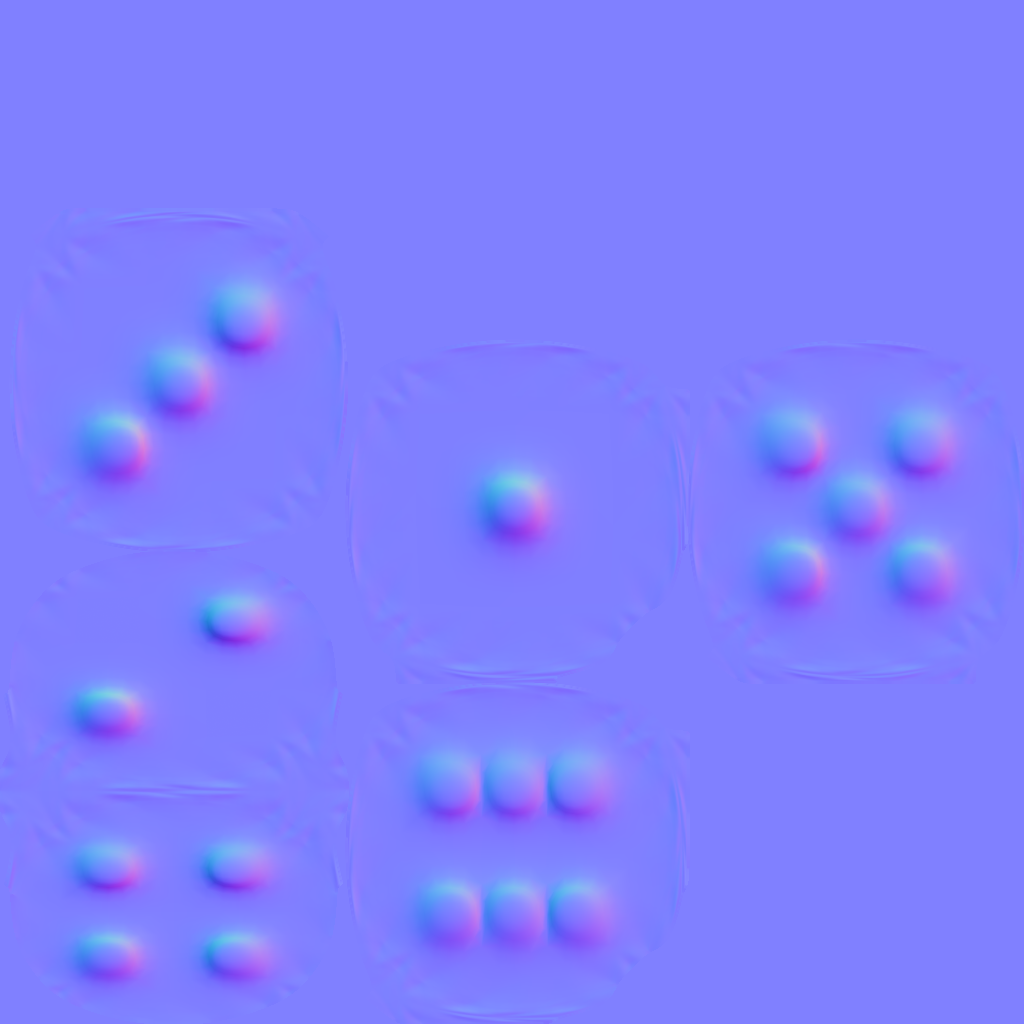
\includegraphics[width=0.49\textwidth]{images/normal_map}
    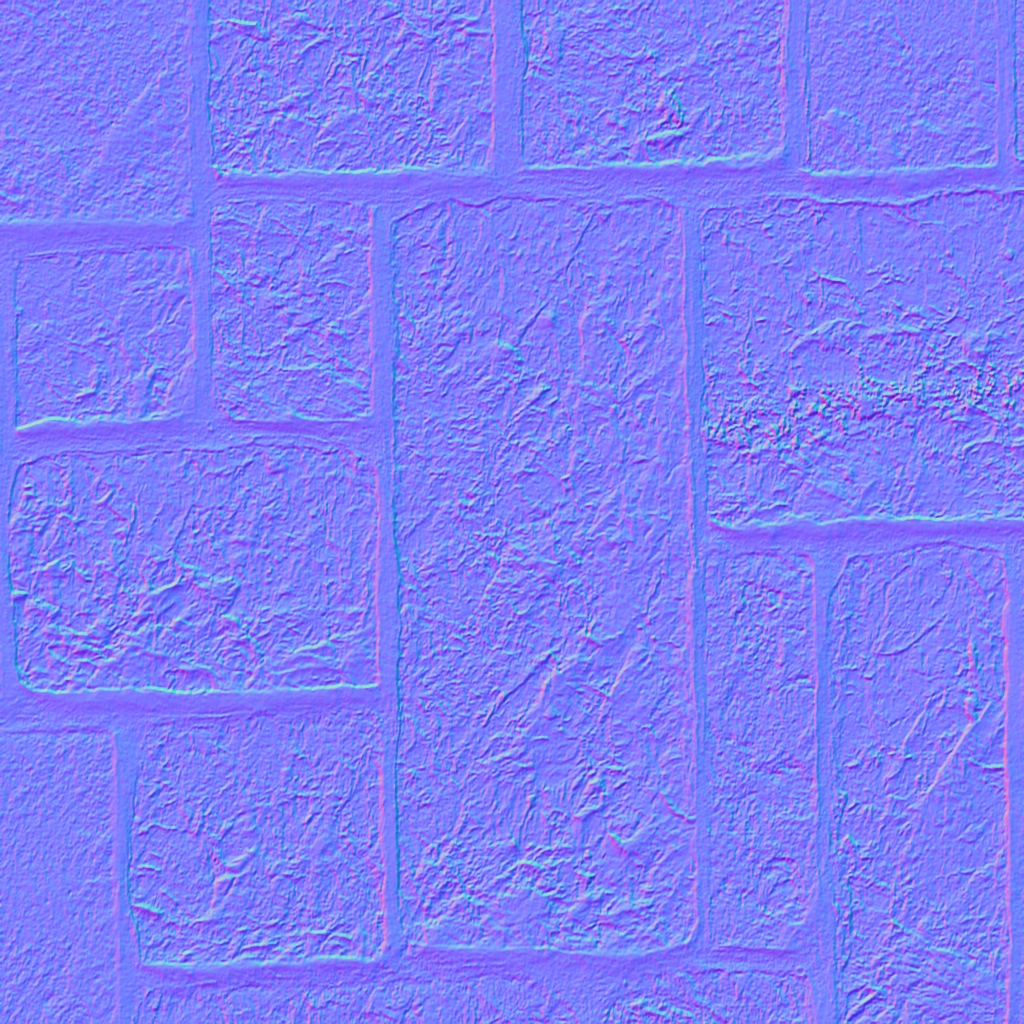
\includegraphics[width=0.49\textwidth]{images/normal_map2}
  \end{center}
  \caption{Quelques normal maps utilisées dans ce TP.}
  \label{fig:normalmap}
\end{figure}          
%>>>

% - Exercices Bonus <<<1
\section{Exercices Bonus}
\label{sec:exercices_bonus}

Les exercices suivant ne sont pas obligatoires. Ils sont suffisamment fun pour que vous preniez le temps de les faire. 

% -- Exercice 6 <<<1
\subsection{Exercice 6}
\label{sec:exercice_6}
Ajouter une (ou plusieurs) source de lumière de type spot et faites la balayer
la scène en fonction du temps (cf figure \ref{fig:spot}).


\begin{figure}
  \begin{center}
    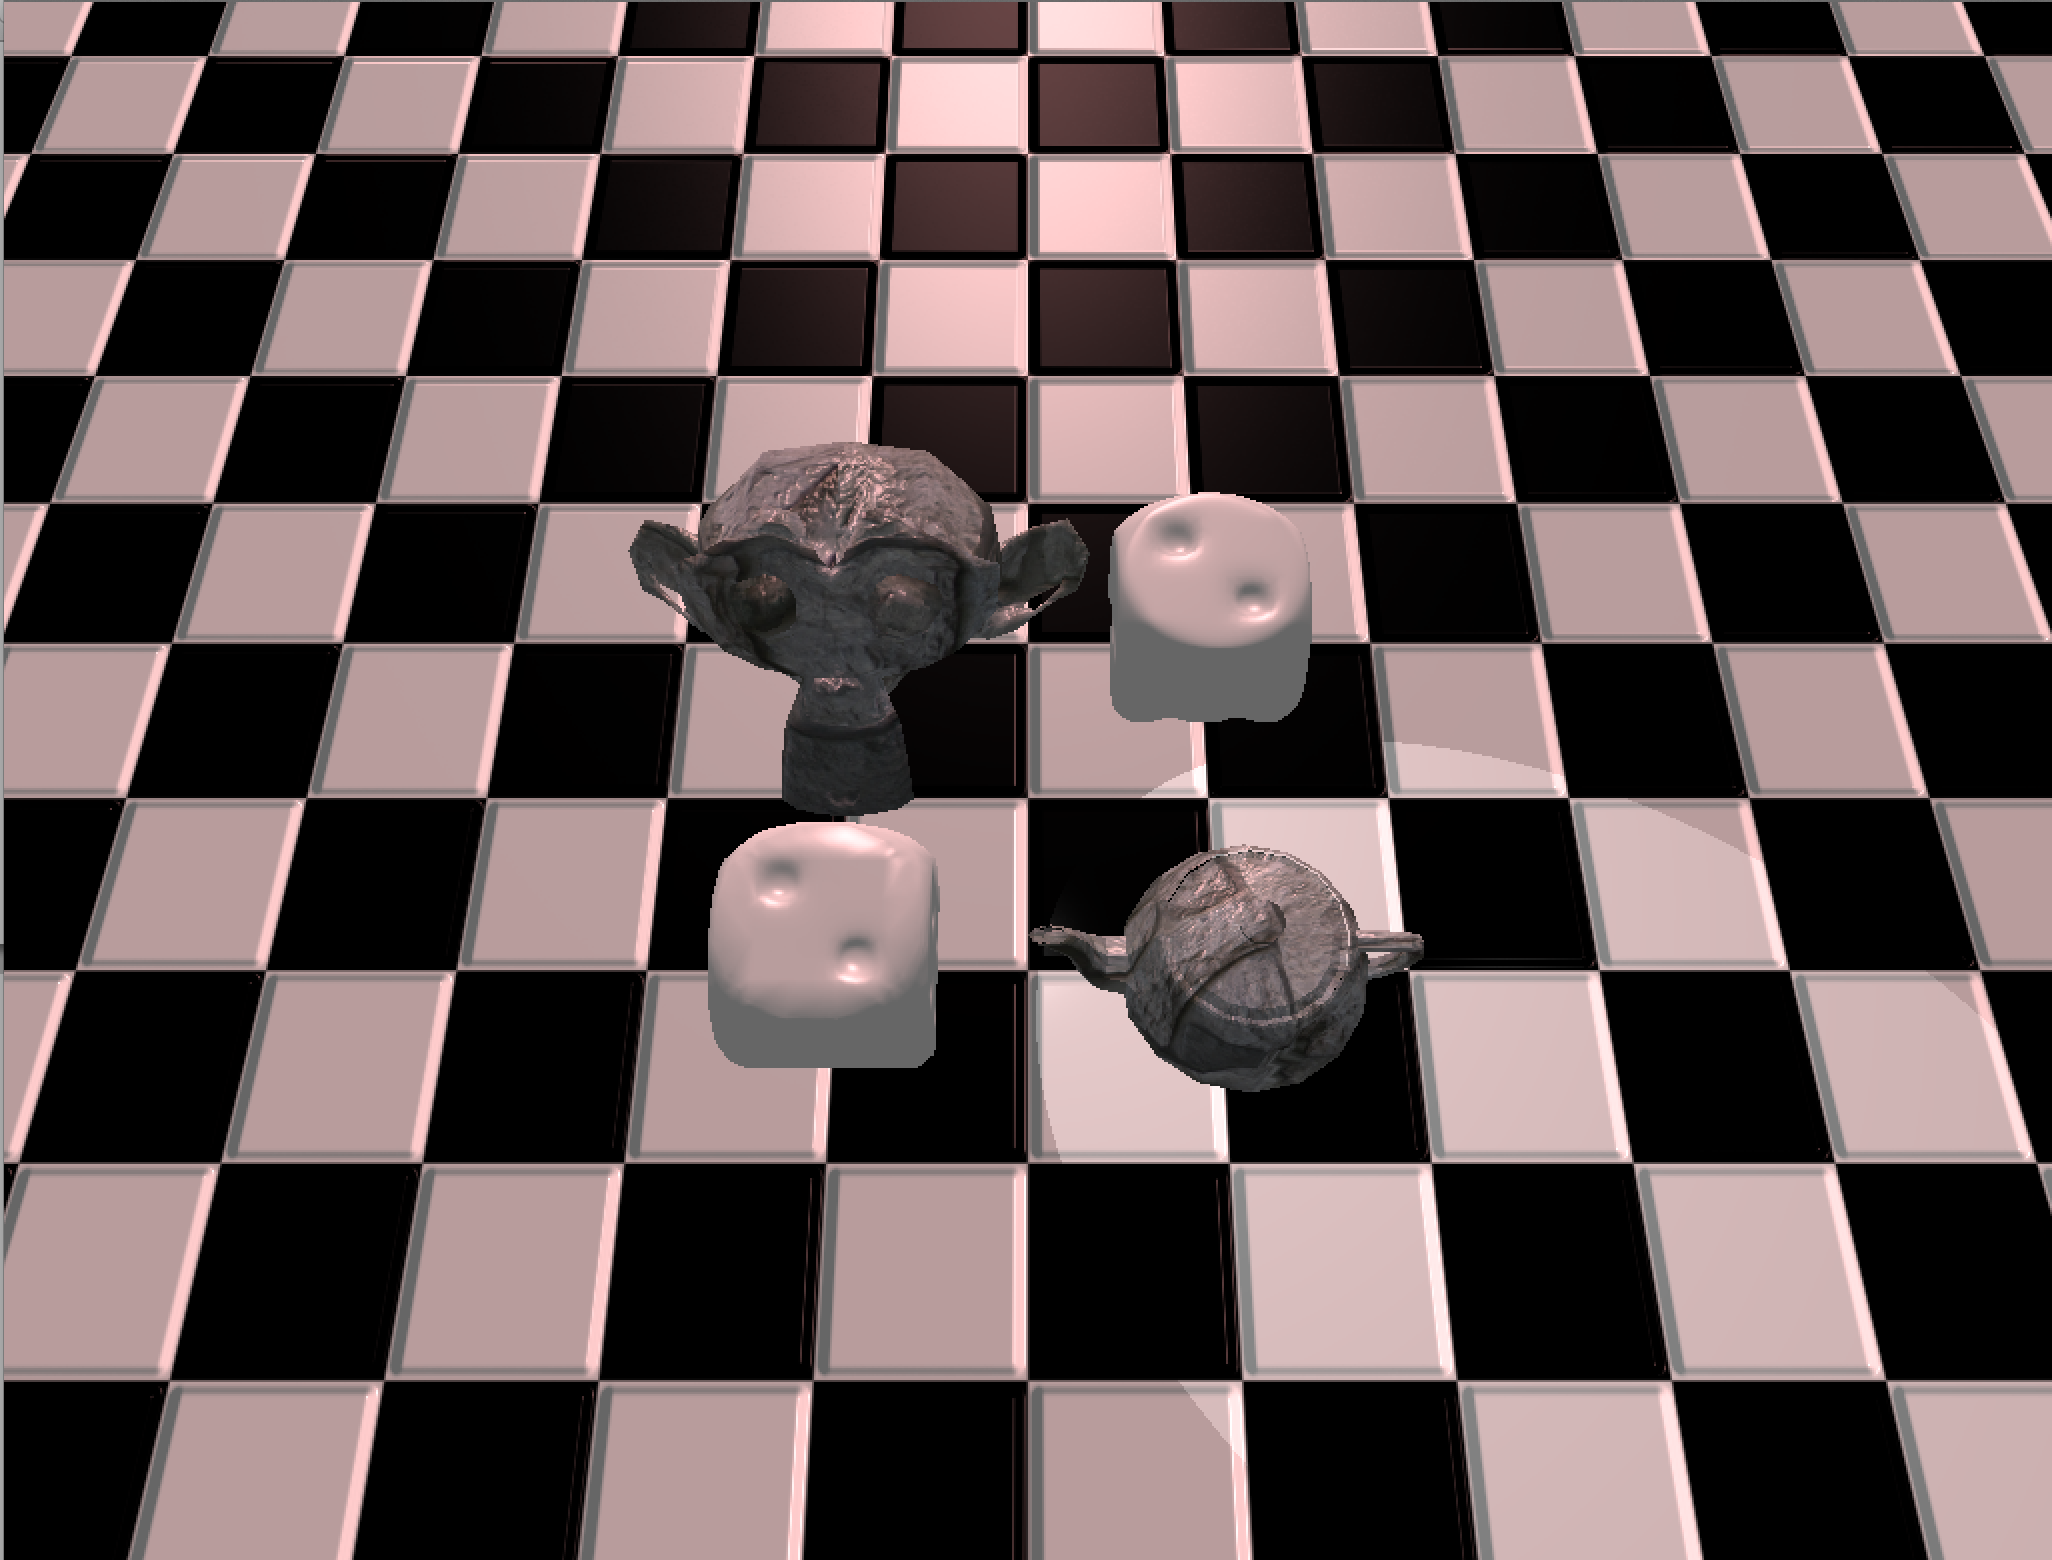
\includegraphics[width=0.49\textwidth]{images/spot}
    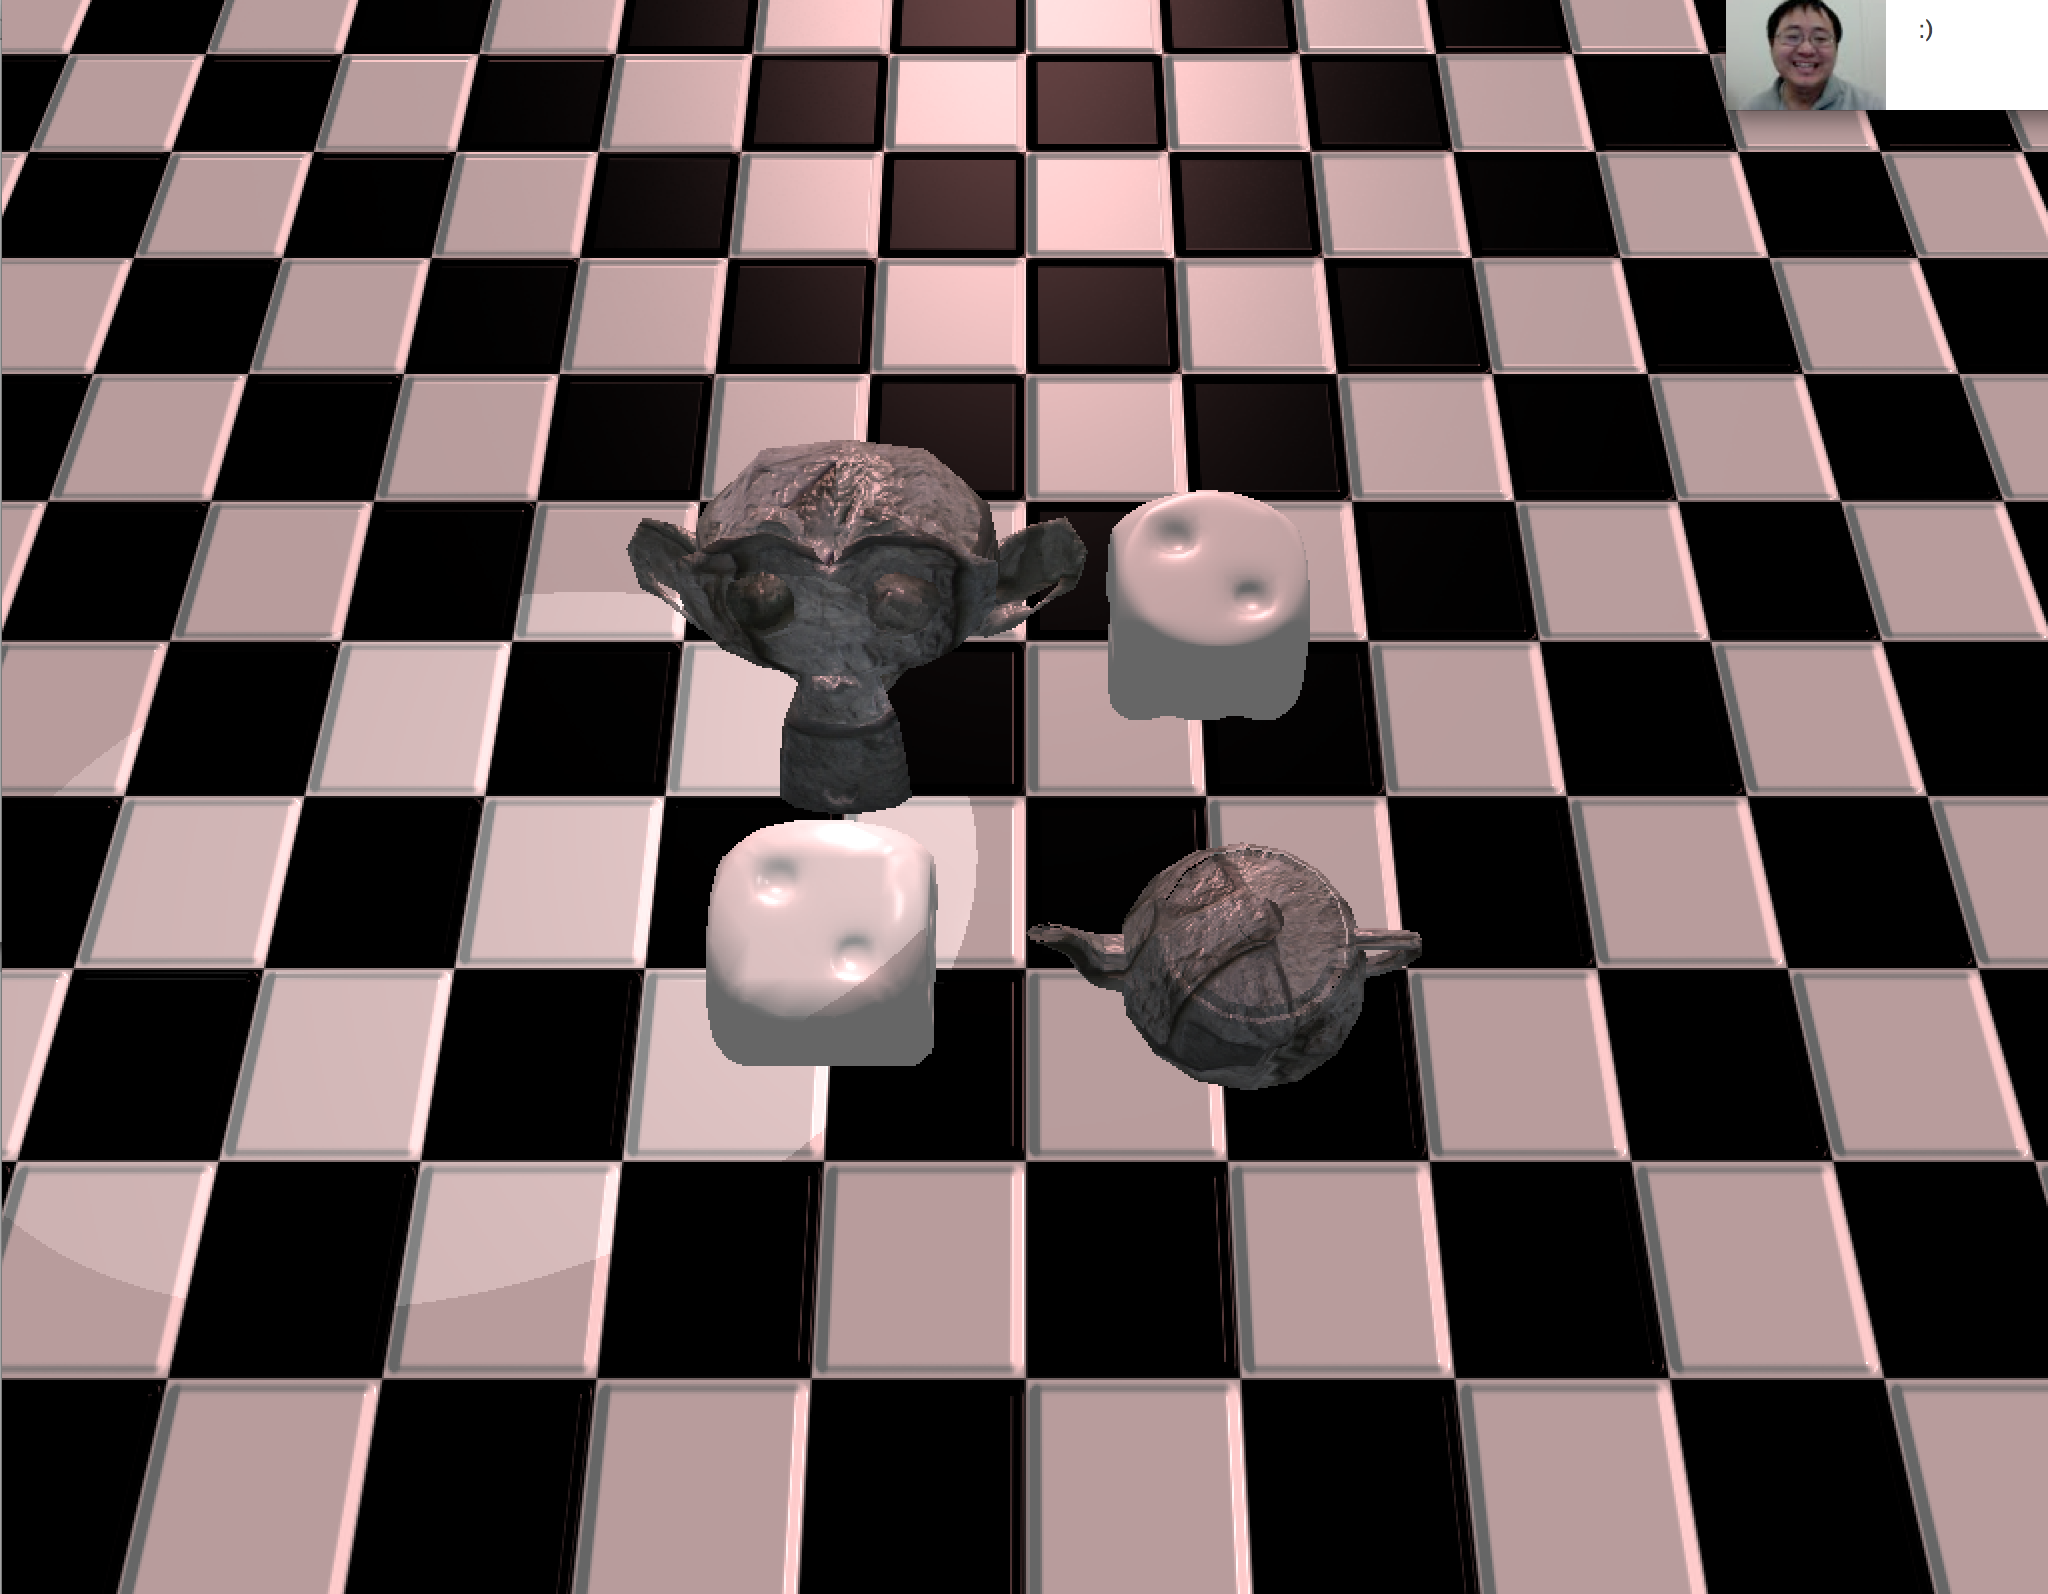
\includegraphics[width=0.49\textwidth]{images/spot2}
  \end{center}
  \caption{Screenshots du spot balayant la scene.}
  \label{fig:spot}
\end{figure}          

% -- Exercice 7 <<<1
\subsection{Exercice 7}
\label{sec:exercice_7}

Une autre normal map provenant de
\url{http://kay-vriend.blogspot.fr/2012/11/well-preserved-chesterfield.html} est
fournie dans votre répertoire. D'autres types de carte sont fournis sur cette
même page. Utilisez les pour implémenter des techniques parmi les suivantes:

\begin{itemize}
  \item Environment occlusion mapping (facile),
  \item Specular mapping (facile),
  \item Displacement mapping (difficile mais cool).
\end{itemize}


\end{document}

% vim: fileencoding=utf-8 spelllang=fr:
